% % -----------------------------------------------------------------------------
\section{Overview of SBOL}
% % -----------------------------------------------------------------------------

Synthetic biology designs can be described using:
\begin{itemize}
\item Structural terms, e.g., a set of annotated sequences or information about the chemical makeup of components.
\item Functional terms, e.g., the way that components might interact with each other and the overall behavior of a design.
\end{itemize}
In broad strokes, the prior SBOL 1.1 standard focused on physical, structural information, whereas SBOL 2.0 extends to also include functional aspects. 
The physical information about a designed genetic construct includes the order of its constituents and their descriptions. The exact locations of these constituents and their sequences allow genetic constructs to be defined unambiguously, and reused in other designs. SBOL 2.0 extends SBOL 1.1 in several ways: it extends physical descriptions to include entities beyond DNA sequences, and it allows for functional descriptions of the design. 

As an example, consider the design of an expression cassette, such as the one found in the plasmid pUC18~\cite{L08752.1}. This device is designed to detect successful versus unsuccessful molecular cloning. 
As an overall system, the device is designed to grow either blue-colored (unsuccessful) or white-colored (successful) colonies in the presence of IPTG and the chemical X-gal. Internally, the device has a number of parts, including a promoter, the lac repressor binding site, and the lacZ coding sequence. 
These parts have specific component-level interactions with IPTG and X-gal, as well as native host gene products, transcriptional machinery and translational machinery that collectively cause the desired system-level behavior. 

Knowledge of how such a device functions within the context of a host and how it might be adapted to new experimental applications has generally been passed on through working with fellow scientists or reading articles in papers and books. 
But there was no systematic way to communicate the integration of sequences with functional designs, so users typically had to look in many different places to develop an understanding of a system.  
The SBOL 2.0 standard allows designers to describe these functional characteristics and connect them to the physical parts and sequences that make up the design. 

SBOL 2.0 includes two main classes that match the structural/functional distinction above:
\begin{itemize}
\item The \sbol{ComponentDefinition} object describes the physical aspects of the designed system, such as the DNA or RNA sequences and the physical relationships among sub-components, such as one sequence containing another as a sub-sequence.
\item The \sbol{ModuleDefinition} object describes interactions of the designed system, such as specific binding relationships and repression and activation relationships. 
\end{itemize}

\ref{images:overview1} shows a simplified view of these classes, as well as other helper classes in SBOL. To continue with the pUC18 example, the description would begin with a top-level \sbol{ModuleDefinition}.  
The \sbol{ModuleDefinition} specifies the structural elements that make up the cassette by referencing a number of \sbol{ComponentDefinition} objects. These would include the DNA component for the promoter and the small molecule component for IPTG, for example.  
The \sbol{ComponentDefinition} objects can be organized hierarchically.  For example, the plasmid \sbol{ComponentDefinition} may reference \sbol{ComponentDefinition}s for the promoter, coding sequence, etc.  
Each \sbol{ComponentDefinition} object can also include the actual \sbol{Sequence} information (if available), as well as \sbol{SequenceAnnotation} objects that identify the locations of the promoters, coding sequences, etc., on the \sbol{Sequence}.  
In order to specify functional information, the \sbol{ModuleDefinition} can specify \sbol{Interaction} objects that describe any qualitative relationships among components, such as how IPTG and X-gal interact with the gene products.  Finally, a \sbol{ModuleDefinition} object can point to a \sbol{Model} object that provides a reference to a complete quantitative model using a language such as SBML, CellML, Matlab, etc.  Finally, all the of elements of the genetic design can be grouped together within a \sbol{Collection}.

\begin{figure}[ht]
\begin{center}
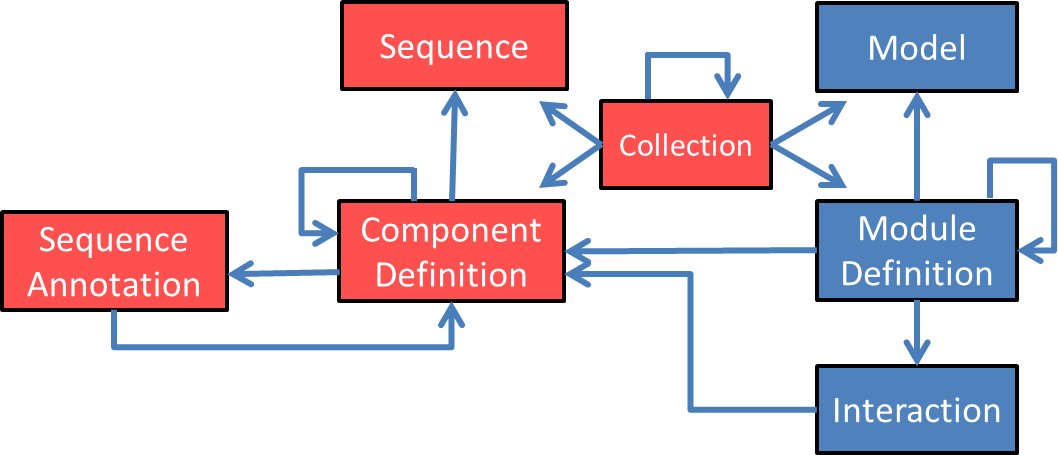
\includegraphics[scale=0.7]{images/OverviewFigforSpec-v7.png}
\caption{Main classes of information represented by the SBOL standard, and their relationships.  Red boxes are classes from the SBOL 1.1 that focused on structure, whereas blue classes are some of the new classes that support the functional aspects of designs.}
\label{images:overview1}
\end{center}
\end{figure}

Whereas \ref{images:overview1} provides a broad overview of SBOL, \ref{images:overview2} provides a detailed, implementation-level overview of the class structure for the SBOL 2.0 data model. This figure relies on the semantics of the \emph{Unified Modeling Language} (UML), which will be presented in more detail in the next section. \ref{images:overview2} distinguishes between \emph{top level} classes, in green, and other supporting classes (note that \ref{images:overview1} also includes all of the top level classes). In \ref{images:overview2}, dashed arcs represent "refersTo", whereas a solid arrow represents ownership. In UML, the meaning of ownership is that if a parent class is deleted, so are all of its owned children. Thus, a \sbol{Collection} does not own its
\sbol{ComponentDefinition} objects, because these can stand on their own. All of the supporting classes (in orange) must be owned by some top-level class, directly or indirectly. 

% Figure~\ref{images:overview2} provides a more detailed view the the class structure for the SBOL 2.0 data model.  The main, or \emph{top level} classes, are \sbol{Collection}, \sbol{ComponentDefinition}, sbol{Sequence}, \sbol{ModuleDefinition}, and \sbol{Model}.  The key distinction of these classes is that they can stand alone and be referenced by other top level objects (see the dashed arrows between the green boxes).  The purpose of these classes is described above.  Each of these classes is assisted in their purpose by several \emph{child} classes.  The key distinction of a child object is that it is owned by its parent object, and if that parent object is removed, so is the child object.  This ownership is indicated using the solid arrows in the figure.  For example, a \sbol{ComponentDefinition} owns its \sbol{SequenceAnnotation}s.  

\begin{figure}[ht]
\begin{center}
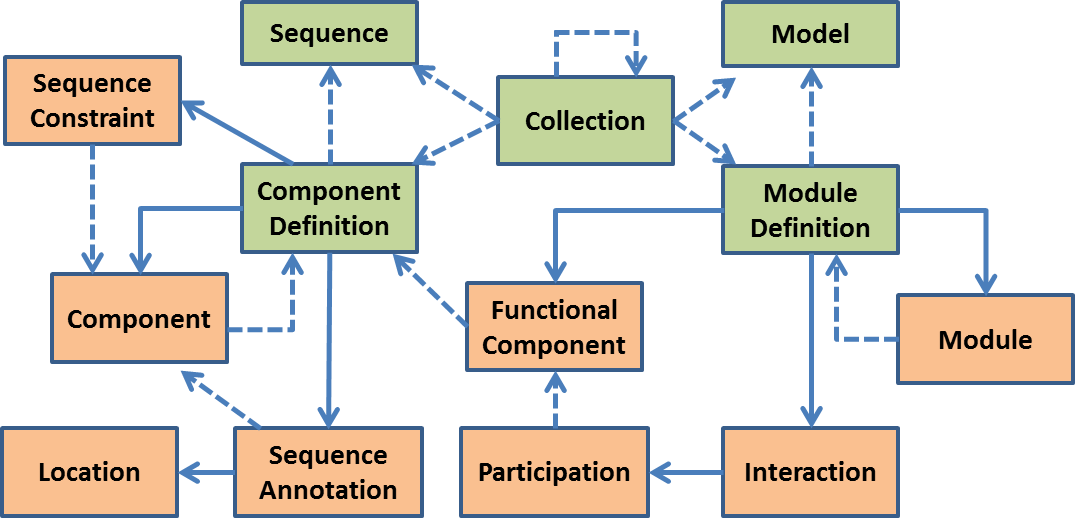
\includegraphics[scale=0.85]{images/OverviewFig2-v4.png}
\caption{Main classes of information represented by the SBOL 2.0 standard, and their relationships.  Green boxes are ``top level'' classes, while the other classes are in support of these classes. Solid arrows indicates ownership, whereas a dashed arrow indicates that one class refers to an object of another class.}
\label{images:overview2}
\end{center}
\end{figure}

The second figure additionally depicts the connection of the functional side (modules) to the physical side (components). 
This is accomplished via the class \sbol{FunctionalComponent}. This class allows modules to own their components instances, and yet also allows the physical descriptions (in \sbol{ComponentDefinition}s) to stand on their own. 
In a similar manner, the ability to have hierarchies of either functional or physical components shown in \ref{images:overview1} must be broken apart, so that sub-components can be used in multiple functional modules or multiple physical components. 
Thus, instead of the arc from \sbol{ModuleDefinition} to itself as in \ref{images:overview1}, our implementation actually divides this notion into two classes, \sbol{ModuleDefinition} and \sbol{Module}. 
Therefore, a \sbol{ModuleDefinition} does not own the \sbol{ModuleDefinition}s that it uses, but instead it refers to them using the \sbol{Module} objects that it does own.  The identical relationship occurs on the physical side with \sbol{ComponentDefinition} and \sbol{Component}. Finally, SBOL 2.0 provides a few other additional helper classes such as \sbol{Location}, which generalizes the positioning information from SBOL 1.1 to allow discontinuous ranges and cuts to be annotated, and \sbol{SequenceConstraint}, which generalizes the relative positioning information among \sbol{Component}s.  There is also 
\sbol{Participation}s, which allow \sbol {Interaction} objects to specify the roles of their participants while referencing the \sbol{FunctionalComponent}s, so that these can stand on their own. Finaly, there is the \sbol{MapsTo} class (not shown) that enables connections to be made between \sbol{Component}s and \sbol{FunctionalComponent}s at various levels of the design hierarchy.  The next section provides complete definitions and details for all of these classes.

\Rtodo{Added mapping of objects from 1.1 to 2.0 using the diagram from the libSBOLj paper.  Needs review. Also not entirely sure this is the right place.  Should we move it to its own section later? -CJM}

Figure~\ref{SBOL1TO2} depicts the mapping between SBOL 1.1 data objects and SBOL 2.0 data objects. Collections of DNA components map to Collections of ComponentDefinitions, among other top level SBOL objects.  DnaComponents map to ComponentDefinitions of type DNA.  DnaSequences map to Sequences using the IUPAC encoding for nucleotide sequences. SequenceAnnotations with precise start and end positions are mapped to SequenceAnnotations with Range Locations, while SequenceAnnotations with imprecise positions are mapped to SequenceAnnotations with GenericLocations. Each Sequence Annotation also maps to a Component, which in SBOL 2.0 represents the instantiation or usage of a given ComponentDefinition. Finally, precedes relationships map to SequenceConstraints that specify precedes restrictions.

\begin{figure*}
\begin{center}
  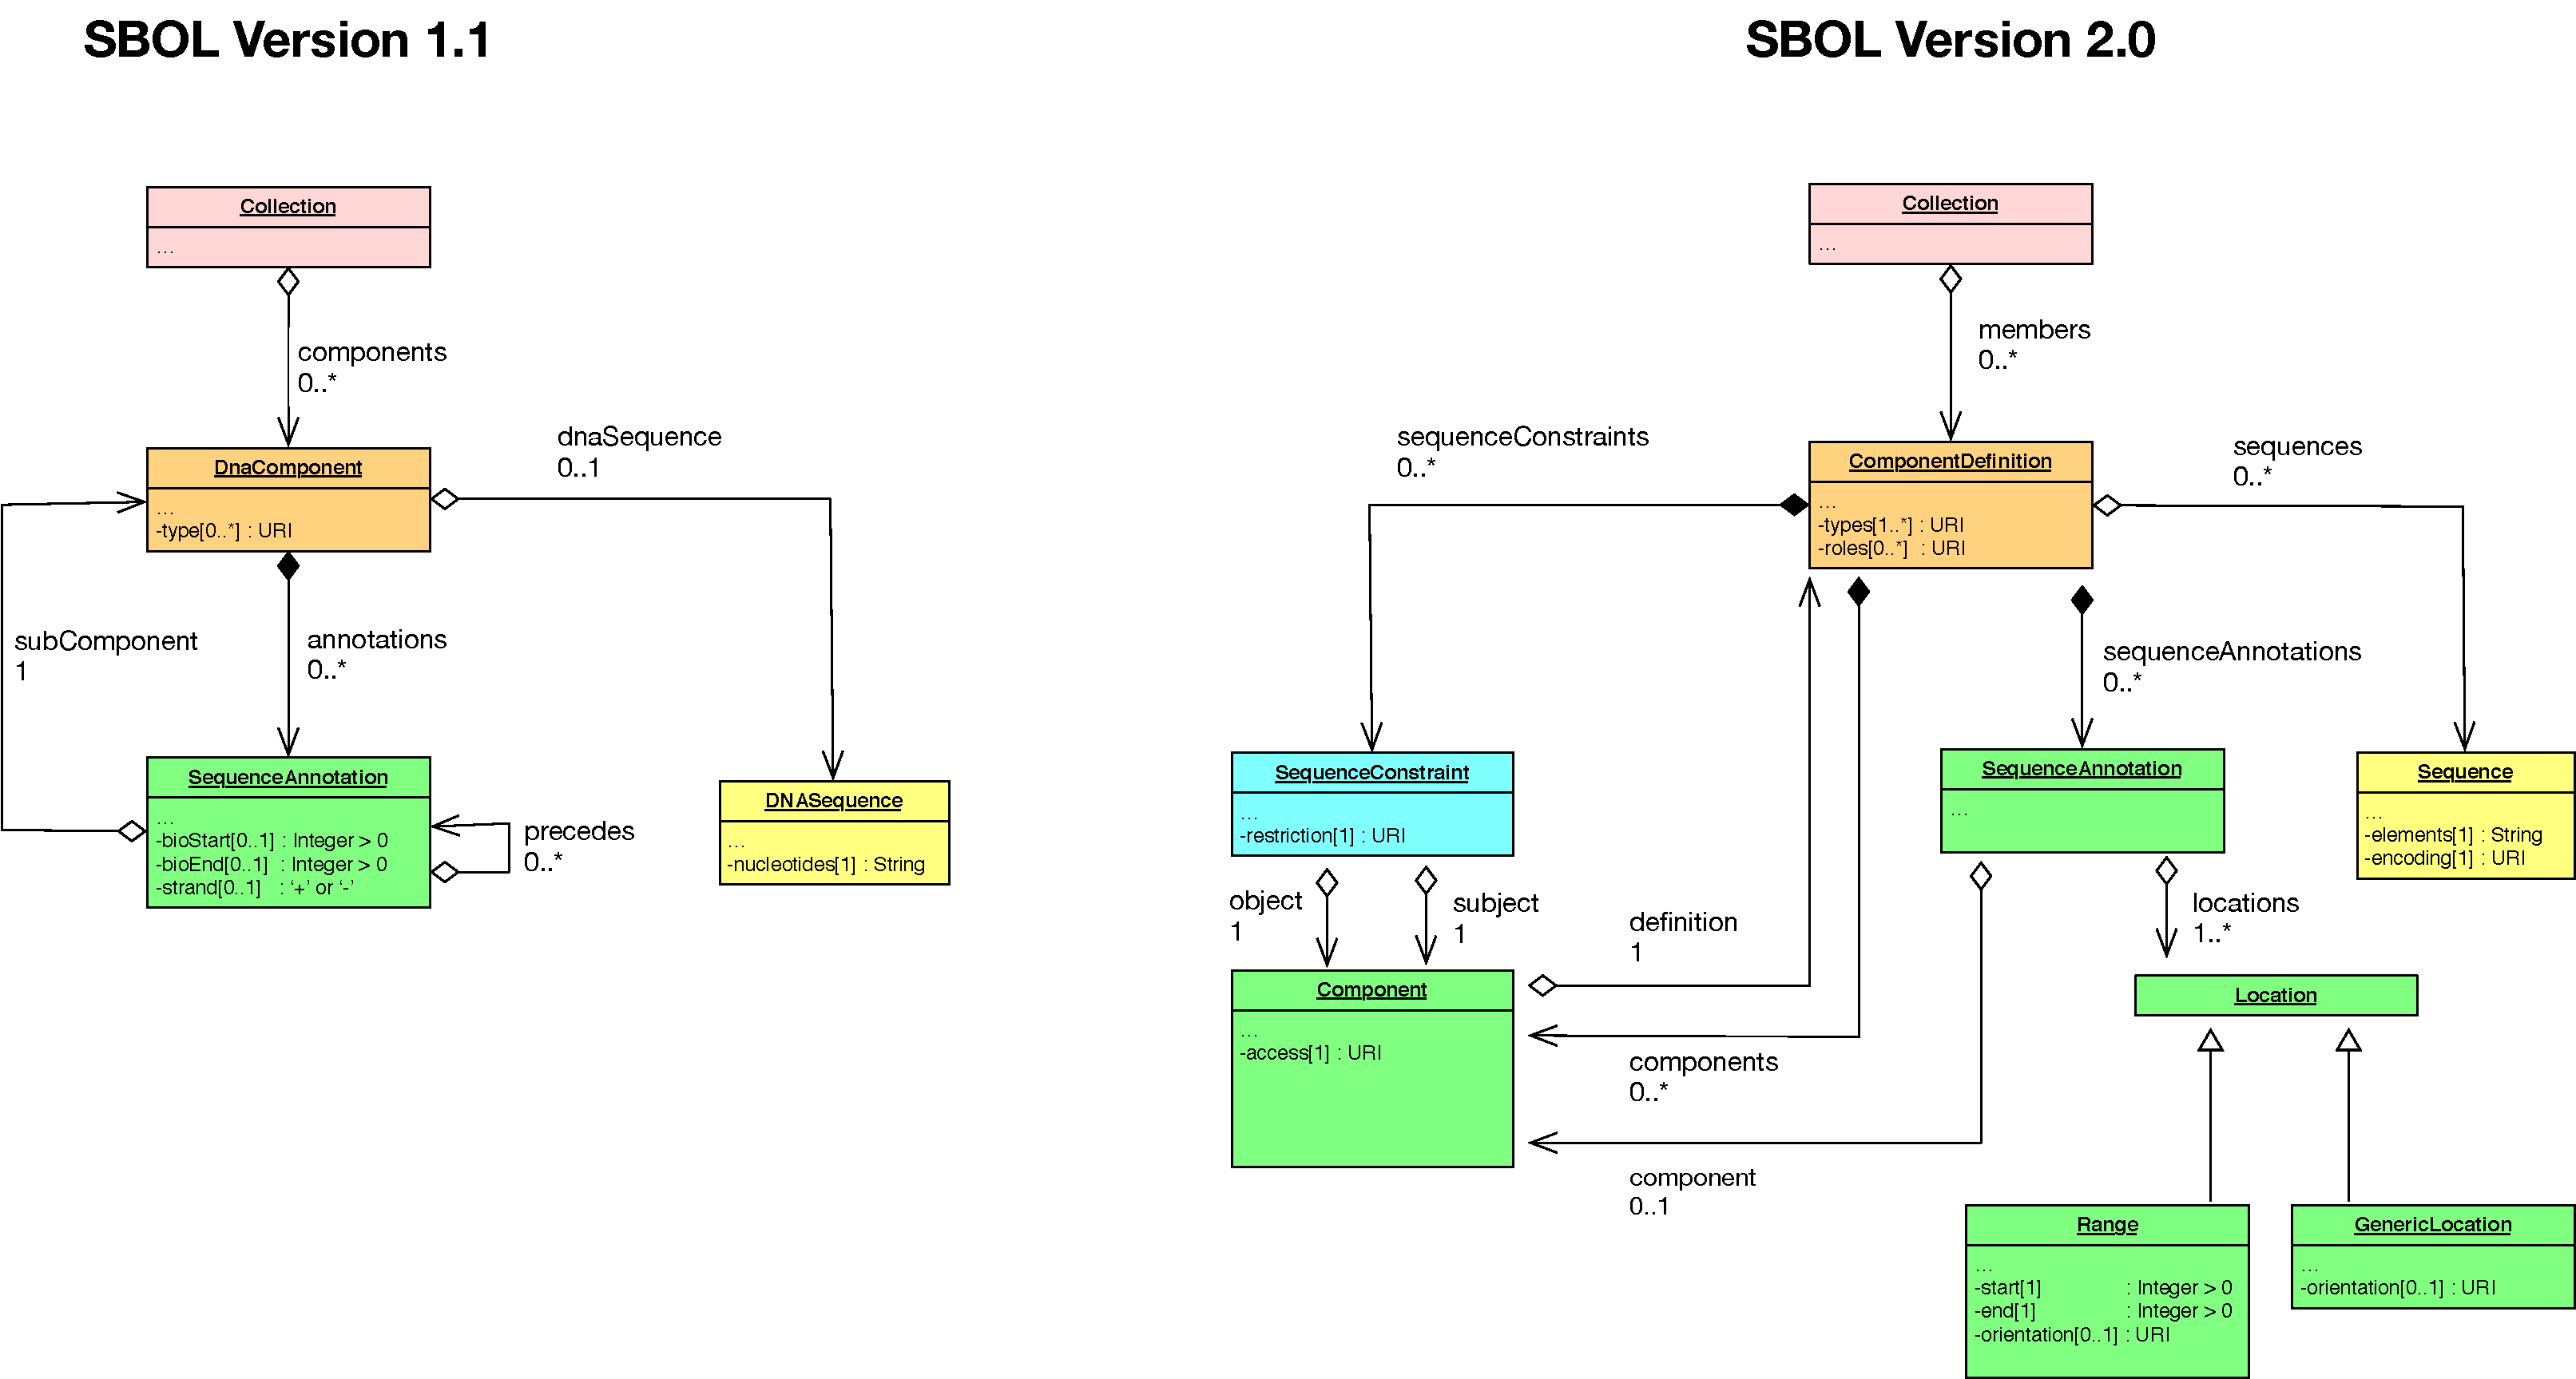
\includegraphics[width=\textwidth]{images/sbol_v1_to_v2} 
\end{center}
\caption{\label{SBOL1TO2}The mapping from the SBOL 1.1 data model to the SBOL 2.0  data model.}
\end{figure*}

There is one final, critical element of SBOL 2.0: its extension mechanism.  This extension mechanism enables the storage of application specific information within an SBOL document.  It is also intended to support the prototyping of data representations whose format is not yet a matter of consensus within the community.  In particular, each SBOL entity can be annotated using the \emph{Resource Description Framework} (RDF). Moreover, application specific entities in the form of RDF documents can be included as \sbol{GenericTopLevel} entities. SBOL libraries make these annotations and entities available to tools as generic properties and objects that are preserved during subsequent read and write operations.

